\section{Introduction} 
\label{sec:introduction}

\begin{quote}
{\em 
The history of all hitherto computer science is (often) the history of a
struggle between isolation, portability and performance. \\ 
(With apologies to Karl Marx.)}
\end{quote}

At the dawn of computing, applications had access to (and had to manage) raw
hardware. Applications were not portable, and isolation between applications was
non-existent. Operating systems emerged and offered a modicum of isolation and
portability.  As users demanded more portability and better isolation across
applications, OSes became more sophisticated, and deep layering became the norm;
e.g., the modern TCP/IP stack is a classic example.  Layering improves the
application's portability across systems and types of  networks, but incurs
well-known performance issues~\cite{dcqcn,netmap}. Soon enough, solutions
like DPDK~\cite{dpdk} and RDMA~\cite{rdma} emerged that traded off some
portability and isolation to provide better performance.  The trend continued
with virtualization, which offers even more isolation, and additional
portability (e.g., you can pack up and move VMs at will, even live-migrate
them). In return, performance -- especially the network performance is further
reduced~\cite{netvm}. Numerous technologies have been proposed to remedy the
situation (e.g.,~\cite{sriov,netvm,netmap,dpdk}) -- again at the cost of
isolation and portability.

The latest step in this trend is {\em containerization}~\cite{docker,kubernetes,coreos}.  By wrapping
a process into a complete filesystem and namespace cell, a container has
everything needed to run the process, including executables, libraries and
system tools.  A container has no external dependencies, which makes it highly
portable. The namespace of the container is isolated from other containers,
eliminating worries about naming and version conflicts.  Such portability and
independence significantly simplifies the life cycle of a containerized
application, from testing to high availability maintenance. 

\begin{figure}[th]
     \centering 
     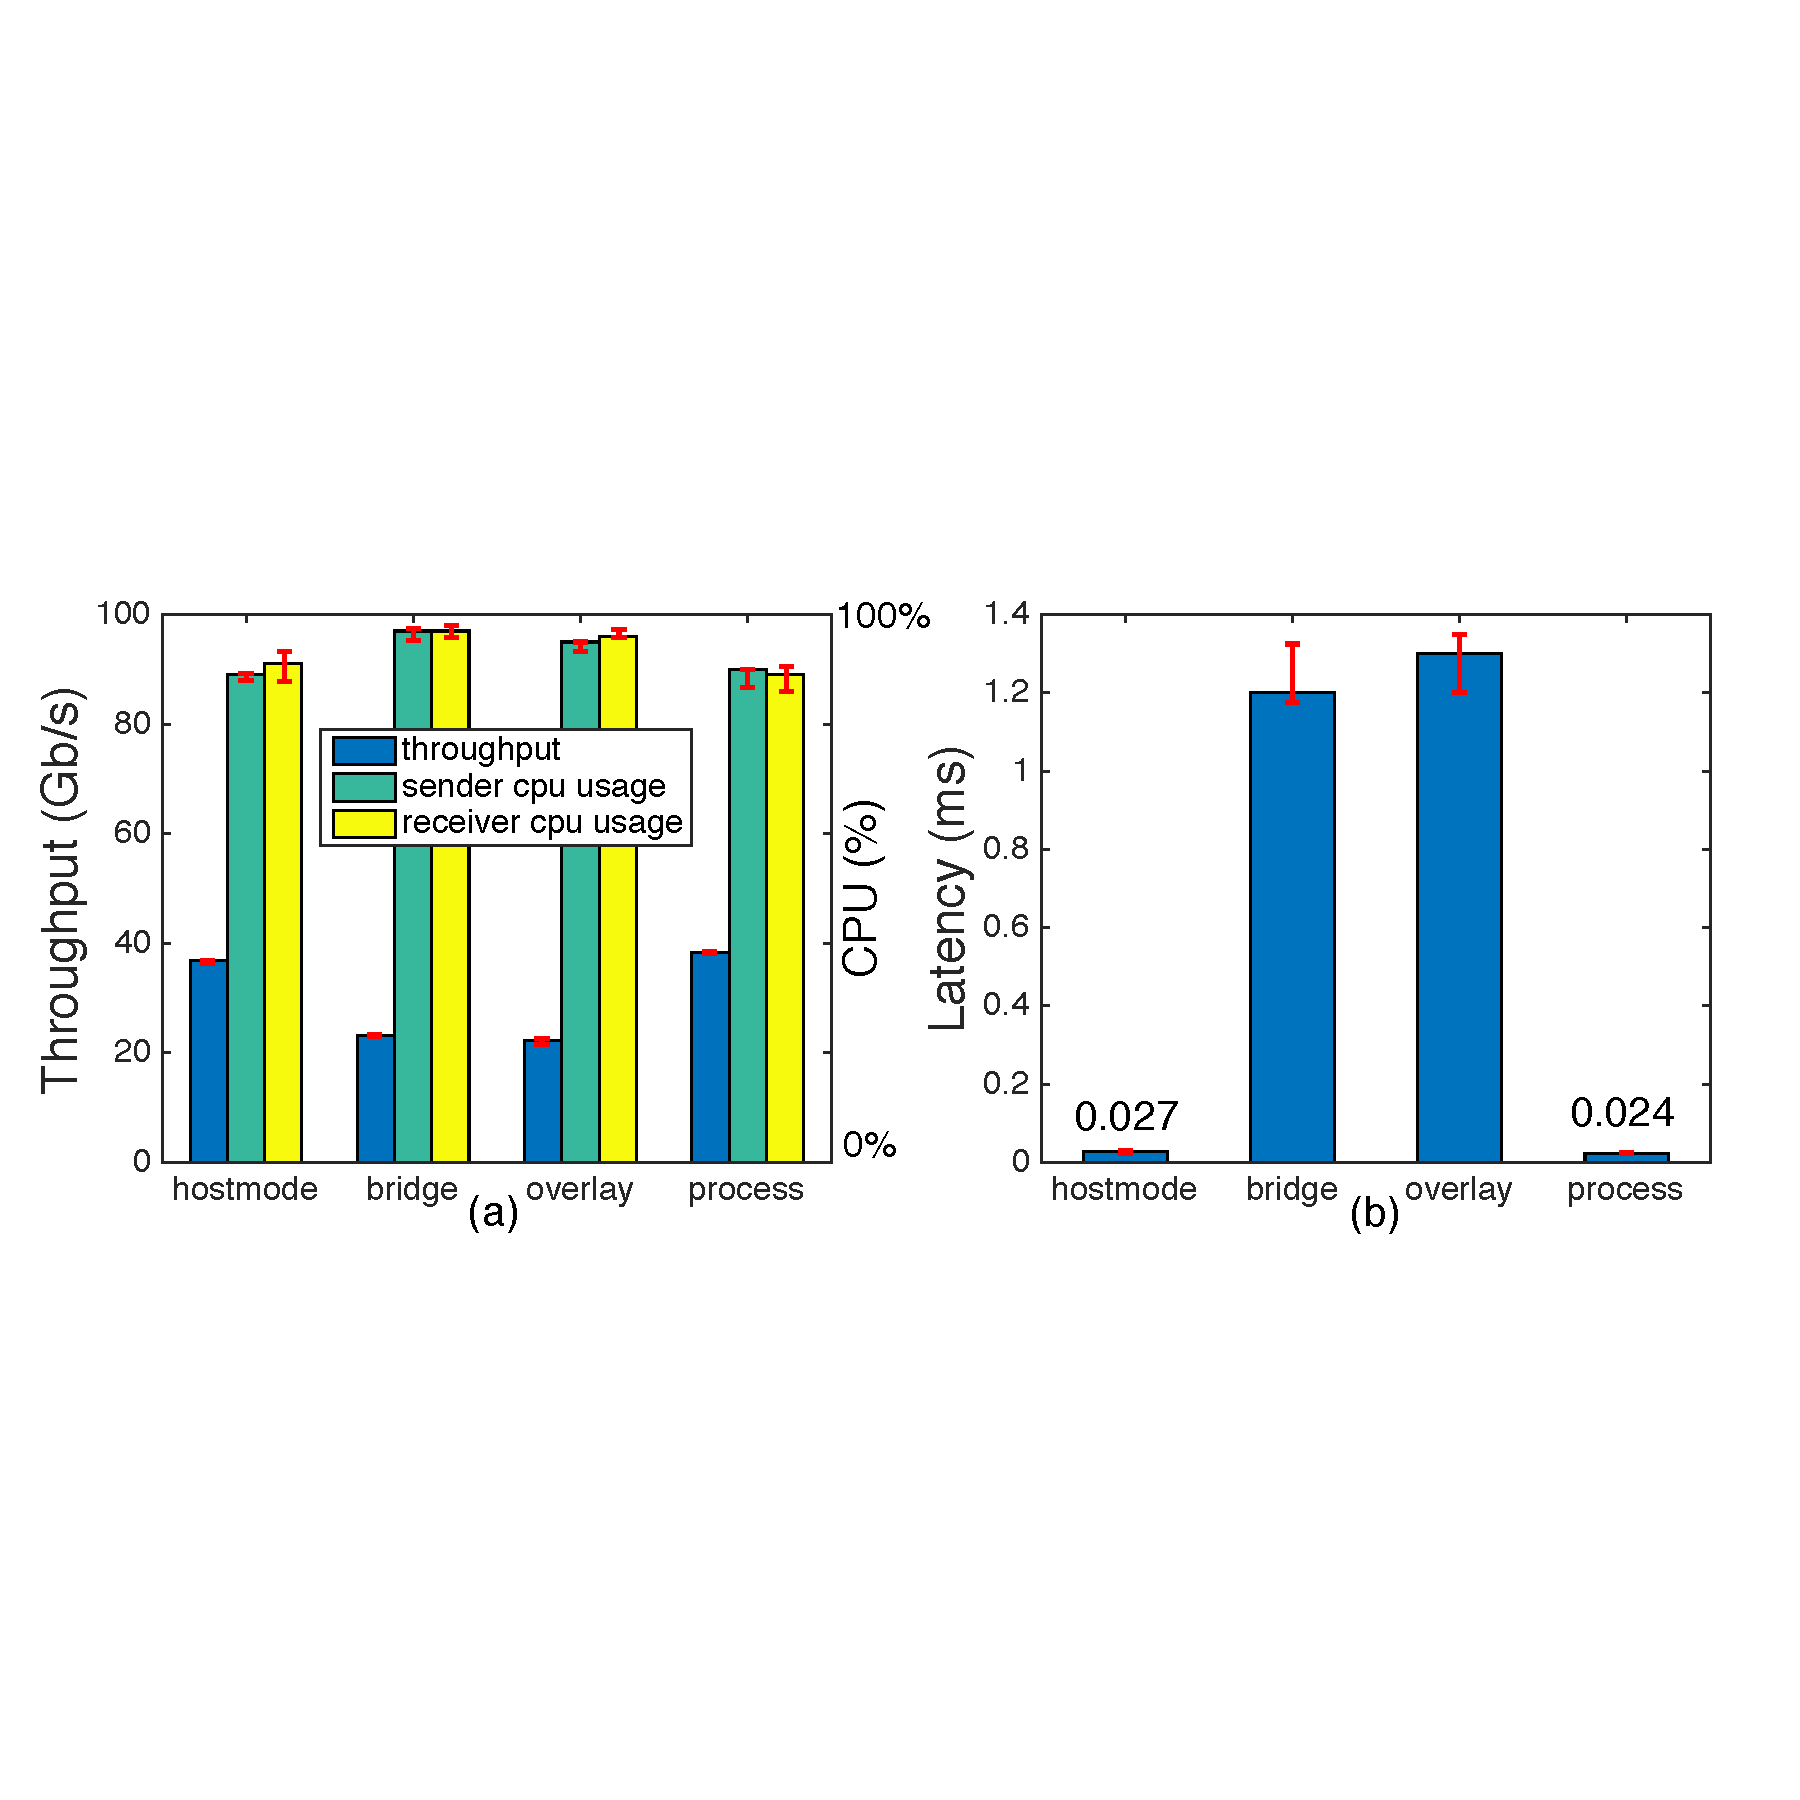
\includegraphics[width=0.5\textwidth]{figures/intro/intro_exist2.pdf} 
     \caption{Performance of two modes of container networking, compared to
     shared memory IPC.} 
     \label{fig:three_modes} 
\end{figure} 
\begin{figure*} [t]
	\centering   
	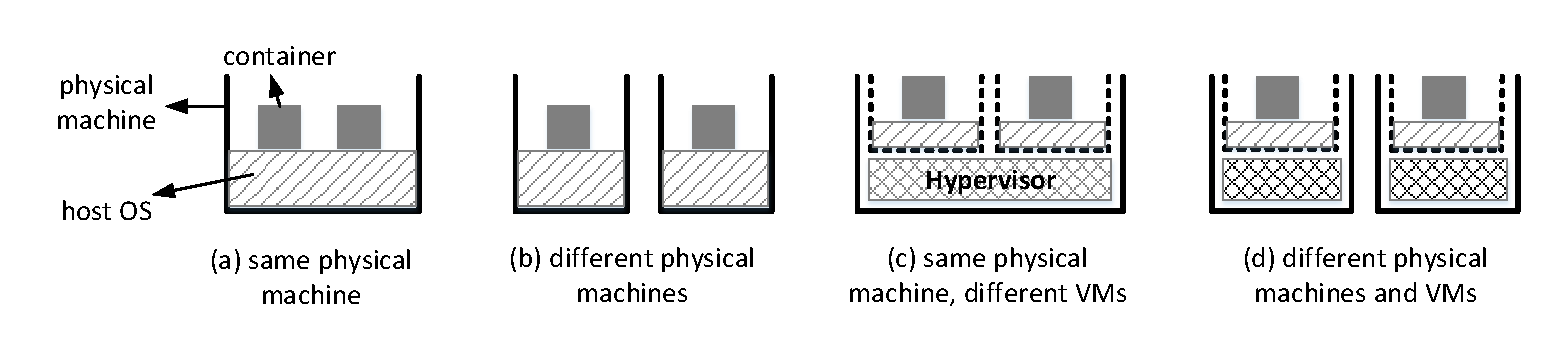
\includegraphics[width=6.7in]{figures/deployment-cases.pdf}   
	\caption{\label{fig:deploy-cases} Representative running environments of containers.}   
\end{figure*}

Unfortunately, containers too suffer the veritable curse of having to sacrifice
one or more of performance, isolation, and portability.  To understand these
potential performance bottlenecks, we set up a simple experiment (more details
in Section~\ref{sec:background}).  We set up two Docker containers on a server
(Intel Xeon E5-2609 2.40GHz 4-cores CPU, 67 GB of memory, 40Gbps Mellanox CX3 NIC,
CentOS 7). We consider three ways for the containers to communicate with each
other: (1) {\em Shared Memory:} This requires special setup\footnote{We 
setup the shared memory data transfer through \texttt{shared memory object} in
shared IPC namespace and measuring the time to pass the pointer and make one copy
of the data.}, to bypass the
namespace isolation, and offers the least isolation, and the least portability;
(2) {\em Host  mode} in which one container binds an interface and a port on the
host and use the host's IP to communicate, like an ordinary process and hence
are not truly isolated as they must share the port space; and (3)  {\em Overlay
mode} in which the host runs a software router which connects all containers on
the host via a bridge network and the software routers enable overlay routing
across multiple hosts to enable maximum portability as  each container can even
have public IPs assigned.

Figure~\ref{fig:three_modes} is a telling demonstration of the fundamental
tussle between portability, isolation, and performance. We make two
observations from this figure. First, that the throughput and latency of both
modes of inter-container communication is significantly worse than
shared-memory IPC. The reason is obvious: the container communication takes a
``hairpin'' path through the full TCP/IP stack. Second, the performance of
overlay networking is worse than host mode. The reason, again, is simple: in
case of overlay networking, hairpinning happens twice, since the packets must
traverse through the software router as well. This figure thus clearly
illustrates the performance cost of isolation and portability.

As the popularity of container networking grows, this inefficiency must be
addressed. On one hand, the low throughput and high latency directly impacts the
overall performance of large scale distributed systems, such as big data
analytics~\cite{varys,orchestra,reining,chowdhury}, key-value
store~\cite{farm}, machine learning, etc. On the other hand,
it forces the applications to reserve substantial CPU resources to merely
perform traffic processing, which significantly raise the cost of running the
applications.

One may argue that there is nothing new here: virtualization suffers from
similar inefficiencies and we know how to address them using techniques like
SR-IOV~\cite{sriov} and NetVM~\cite{netvm}. Unfortunately, these ideas cannot be
directly applied to the container world.  SR-IOV typically scales to tens of VMs
per server. In typical deployments, there are hundreds of containers per server.
The cost of supporting so many containers in the NIC hardware will be
prohibitive.  NetVM~\cite{netvm} cannot be used directly with containers, since
it destroys portability -- it works only when two VMs are on the same server.
Developers prize containers especially for their portability: indeed, one of the
main selling points of containerization is that a containerized application that
runs on developer's desktop will run in the cloud without any changes! 

In this paper we outline a solution to address this issue.  Our ultimate vision
is to develop a container networking solution which provides high throughput,
low latency and negligible overhead and fully preserves container portability in
a manner that is completely transparent to application developers. 

To achieve these seemingly conflicting goals, we observe an opportunity to
leverage two key aspects of typical container deployments: (1) they are
typically managed by a central orchestrator (E.g., Mesos, YARN and Kubernetes
\cite{mesos,yarn,kubernetes}) and (2) are typically deployed over managed network
fabrics (e.g., a public cloud provider). Taking advantage of these easily
available additional bits of information, we sketch a roadmap for an
overlay-based solution  that obtains the relevant deployment-specific
information from the aforementioned container orchestrator and fabric manager
and use this in conjunction with the "right" I/O mechanism (e.g., shared memory
when containers are co-located, vs. RDMA when they are not). 

While this sounds conceptually simple, there are several architectural
and system design challenges in realizing this vision in practice. In the rest
of the paper, we discuss these challenges and sketch a preliminary design. We
will also present results from an early prototype.
